%%%%%%%%%%%%%%%%%%%%%%%%%%%%
% SECTION                  %
%%%%%%%%%%%%%%%%%%%%%%%%%%%%
\vspace{1em}
Le premier mois de mon stage, passé en immersion au sein de l'Agence et aux côtés des membres du SOC-MC, m'a permis d'observer et de comprendre le fonctionnement et l'enjeu des données ainsi que des systèmes sur lesquels j'allais travailler. A la suite des recommandations des analystes du SOC-MC et autres entretiens avec Bruno VALENTIN et Sébastien ABBONDANZA, un premier cahier des charges des besoins a été établi. Cette documentation a servi de base au développement d'un outil qui contribuera à améliorer le processus actuel de mise à jour des règles en répondant aux besoins définis ci-après :\\

\begin{itemize}[itemsep=1em]
    \item[•] L'outil doit être capable de récupérer et de centraliser toutes les règles, quelle que soit leur source (partenaires de CTI ou internes) ;
    \item[•] L'outil doit vérifier la conformité des règles récupérées avec les sondes utilisées et supprimer toute règle dupliquée ;
    \item[•] L'outil devra créer des fichiers de règles portant un nom unique pour chaque sonde ;
    \item[•] L'outil permettra aux analystes du SOC-MC de spécifier des règles à modifier ou à supprimer avant de les envoyer aux sondes ;
    \item[•] L'outil devra rendre compte des résultats du programme.\\
\end{itemize}

L'objectif de cet outil est de répondre à une partie des problèmes énoncés dans ma problématique et à ceux de l'Agence. Le choix technologique de développement de l'outil s'est porté sur le langage de programmation python. L'outil aurait pu être développé à l'aide d'autres technologies, mais Python a été choisi pour la facilité d'utilisation qu'il offre dans la production de scripts facilement exportables. De plus, ce langage me fut suggéré car il est également maîtrisé par la majorité de mes collègues au sein de l'AMSN, ce qui permet à mon travail d'être facilement relu et repris par d'autres personnes au sein de l'Agence.\\

\newpage

Le diagramme de flux de l'outil développé, qui sera analysé en détail dans la suite de mon argumentaire, est le suivant :\\

\begin{figure}[h]%
    \center%
    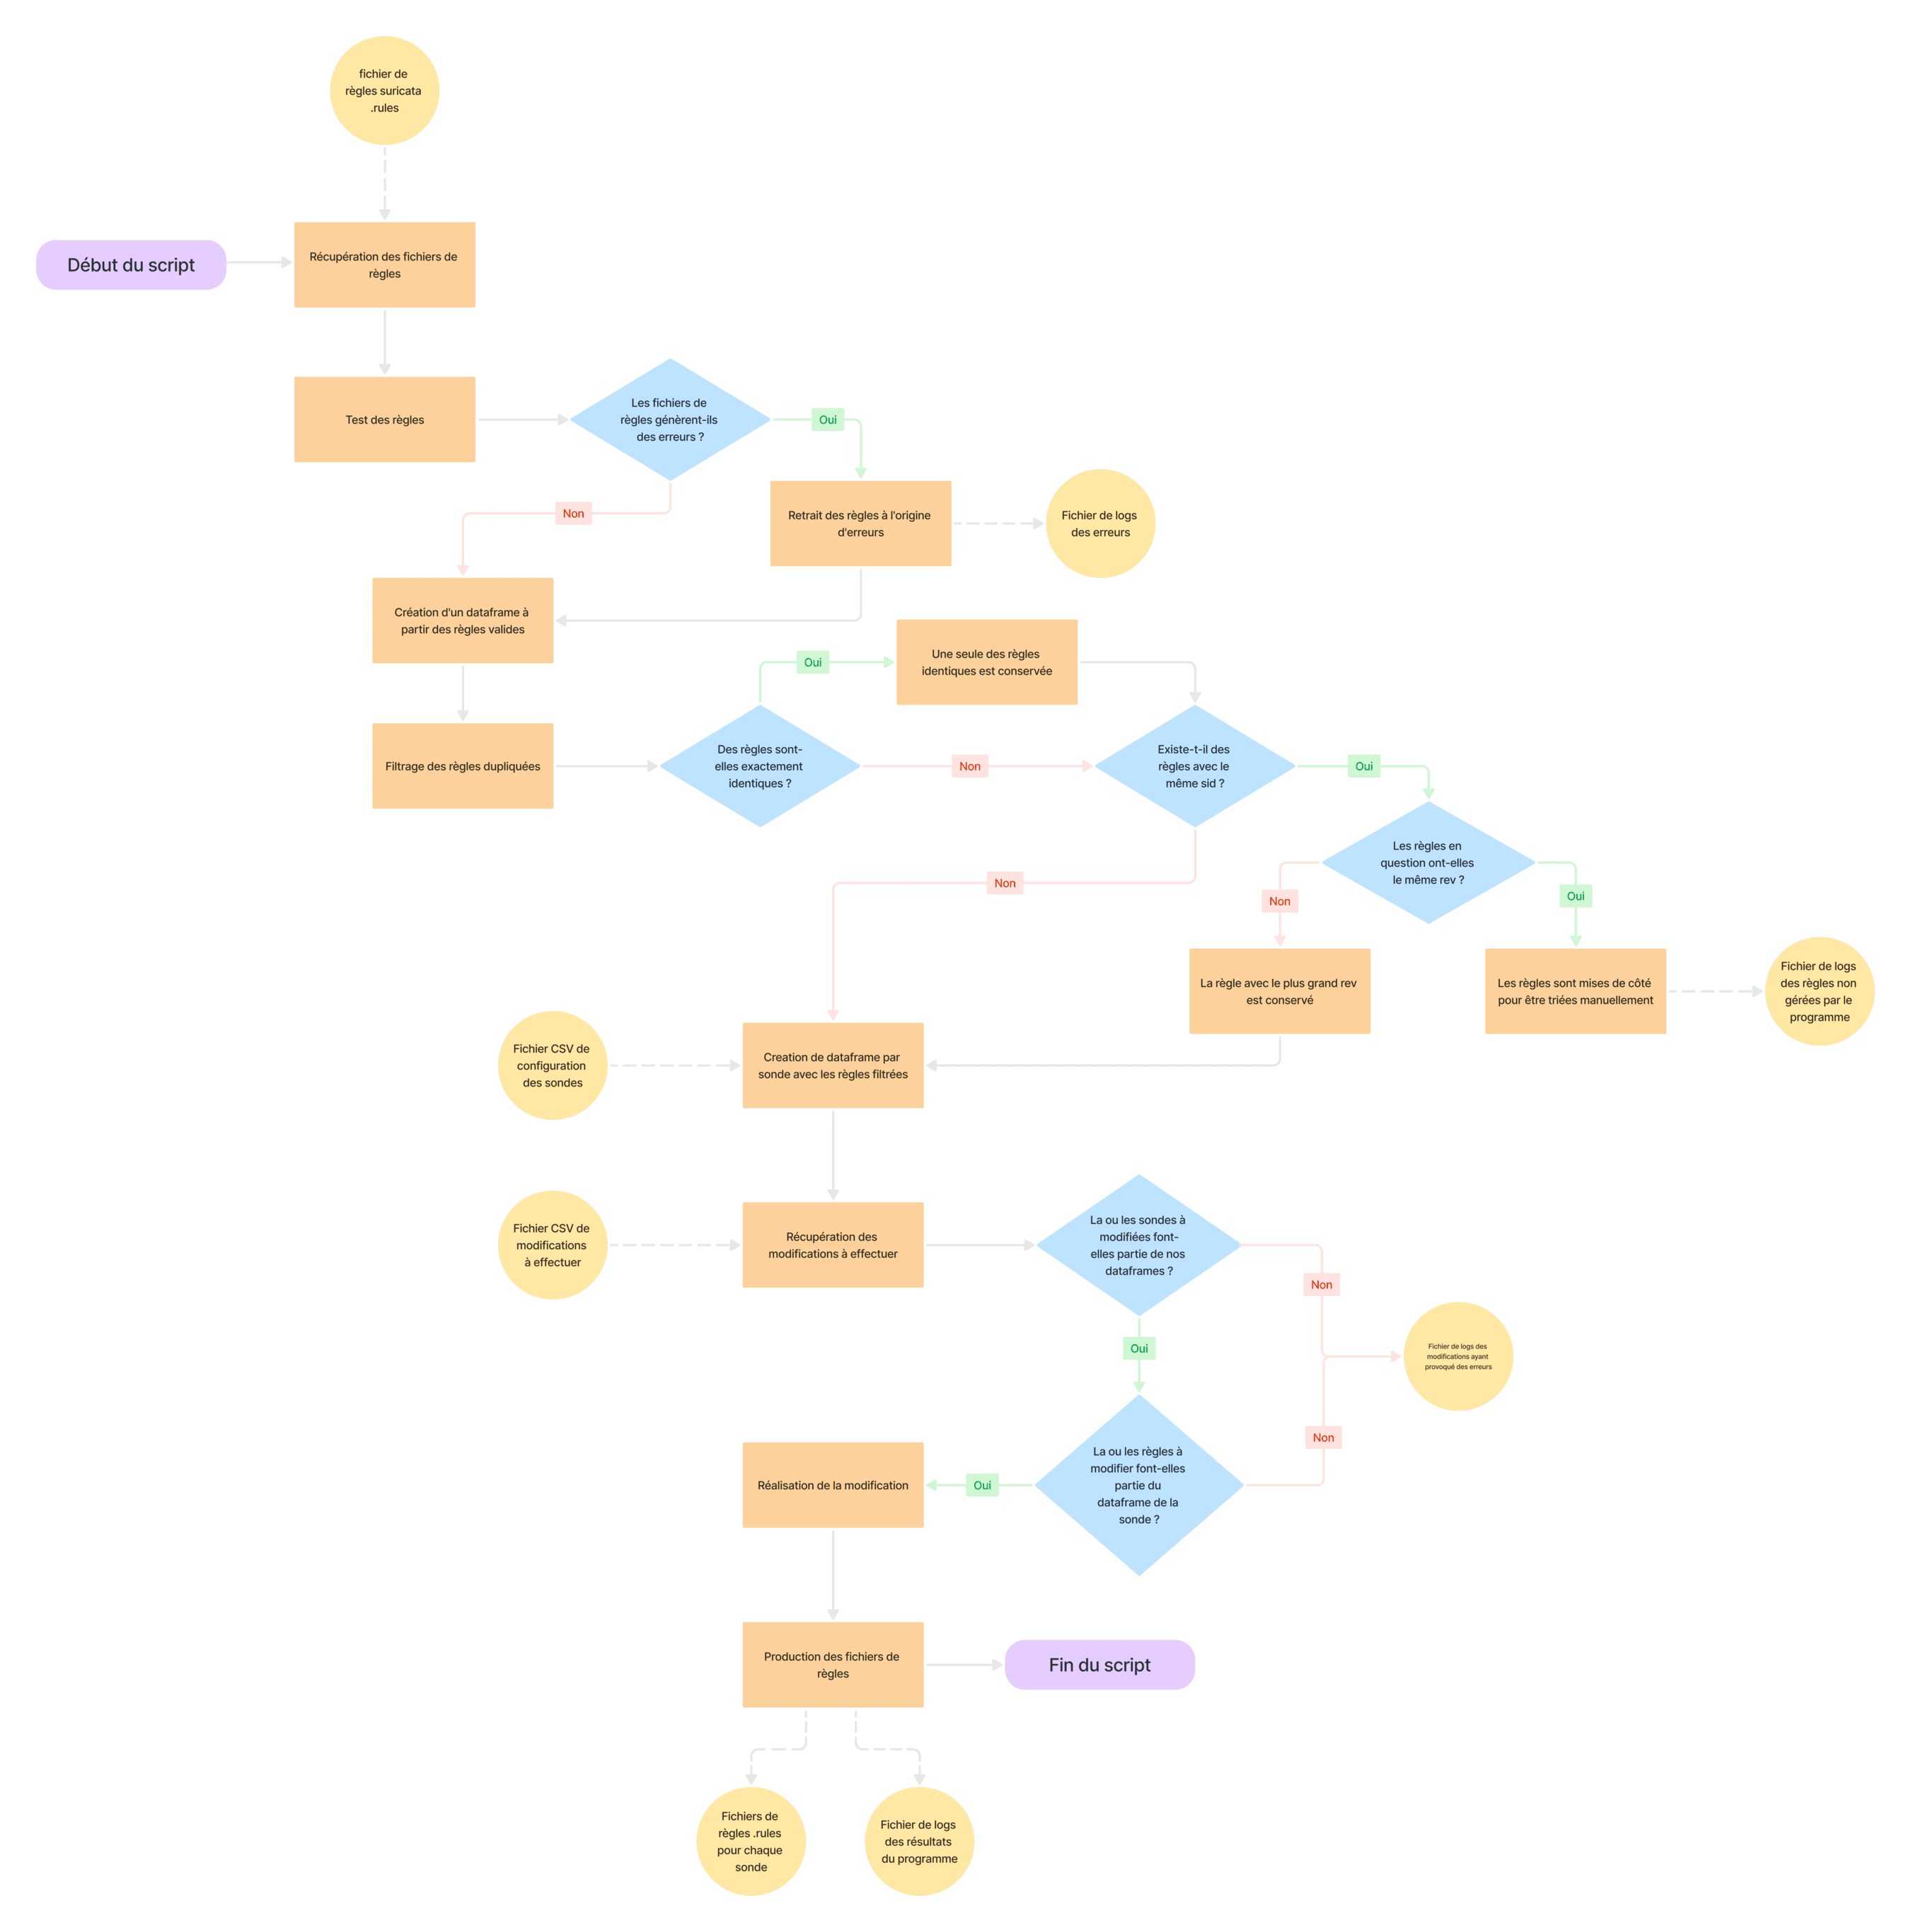
\includegraphics[width=0.97\textwidth]{assets/diagrameFlux.png}
    \caption[Diagramme de flux du programme Python développé]{Diagramme de flux du programme Python développé}\label{fig:diagrameFlux3-1.}
\end{figure}

\newpage

{\fontsize{15pt}{18pt}\selectfont
    \textbf{3.1.0 Suricata}
}

\vspace{1em}

Le programme est conçu pour récupérer les règles de Suricata uniquement. Suricata\footnote{Site officiel de Suricata : \url{https://suricata.io}} est un système de détection d'intrusion (IDS), de prévention d'intrusion (IPS) et de surveillance de la sécurité du réseau (NSM). Créé et maintenu par l'OISF\footnote{Open Information Security Foundation : \url{https://oisf.net/}}, il est utilisé au sein de l'AMSN pour ses fonctions IDS au service des objectifs de détection de l'Agence. Le choix de l'Agence s'est porté sur Suricata car il s'agit du seul outil disponible sur les sondes qualifiées par l'ANSSI.\\

Suricata fonctionne comme un \hyperref[chap2:IDSsignature]{\textbf{\textit{IDS à base de signatures}}} c'est à dire grâce à des signatures pré-configurées, des règles servant à détecter des actions malveillantes réalisées sur un réseau. Les règles Suricata se structurent ainsi en trois parties :
\vspace{0.5em}
\begin{itemize}[itemsep=0.75em]
    \item[•] Une partie \textit{action} qui stipule ce que la règle fera en cas de détection (dans ce cas, où l'Agence ne fait que de la supervision, seule l'action "alerte" est utilisée pour créer des signalements pour le SOC-MC) ;
    \item[•] Un entête dans lequel sont définis le protocole et le réseau sur lesquels la détection aura lieu ;
    \item[•] Une section \textit{option}, qui permet de définir des paramètres variables sur la règle.\\
\end{itemize}

\begin{figure}[h]%
    \center%
    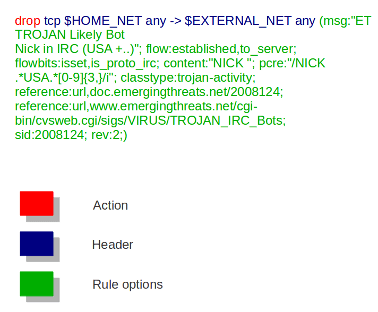
\includegraphics[width=0.5\textwidth]{assets/intro_sig.png}
    \caption[Exemple de la structure d'une règle Suricata (source: \href{https://redmine.openinfosecfoundation.org/projects/suricata/wiki/Suricata_Rules}{redmine.openinfosecfoundation.org})]{Exemple de la structure d'une règle Suricata}\label{fig:intro_sig}
\end{figure}

\newpage

Ces règles sont stockées dans des fichiers de règles \textit{.rules} (un format de fichiers texte utilisé par Suricata), lesquels sont directement fournis par des partenaires de renseignement cyber.\\

\begin{figure}[h]%
    \center%
\begin{lstlisting}[language=Python]
# This Ruleset is EmergingThreats Open optimized for suricata-7.0.3-enhanced.

alert udp $EXTERNAL_NET any -> $HOME_NET 53 (msg:"GPL DNS zone transfer UDP"; content:"|00 00 FC|"; offset:14; reference:cve,1999-0532; reference:nessus,10595; classtype:attempted-recon; sid:2101948; rev:8; metadata:created_at 2010_09_23, cve CVE_1999_0532, updated_at 2019_07_26;)

alert udp $EXTERNAL_NET any -> $HOME_NET 53 (msg:"GPL DNS named version attempt"; content:"|07|version"; offset:12; nocase; content:"|04|bind|00|"; offset:12; nocase; reference:nessus,10028; classtype:attempted-recon; sid:2101616; rev:9; metadata:created_at 2010_09_23, updated_at 2019_07_26;)

alert udp $EXTERNAL_NET any -> $HOME_NET 53 (msg:"GPL DNS named iquery attempt"; content:"|09 80 00 00 00 01 00 00 00 00|"; depth:16; offset:2; reference:bugtraq,134; reference:cve,1999-0009; reference:url,www.rfc-editor.org/rfc/rfc1035.txt; classtype:attempted-recon; sid:2100252; rev:9; metadata:created_at 2010_09_23, cve CVE_1999_0009, updated_at 2019_07_26;)

alert udp $EXTERNAL_NET any -> $HOME_NET 53 (msg:"GPL DNS named authors attempt"; content:"|07|authors"; offset:12; nocase; content:"|04|bind|00|"; offset:12; nocase; reference:nessus,10728; classtype:attempted-recon; sid:2100256; rev:8; metadata:created_at 2010_09_23, updated_at 2019_07_26;)

...
\end{lstlisting}
    \caption[Exemple de fichier de règles (source: \href{https://rules.emergingthreats.net/open/suricata-7.0.3/rules/emerging-dns.rules}{emerging-dns.rules})]{Exemple de fichier de règles}\label{fig:ExampleRulesFile.png}
\end{figure}


\newpage

\subsection{Récupération des règles}

\vspace{1em}

Ces fichiers de règles précédemment cités, sont mis à disposition du programme pour permettre leur centralisation. L'enjeu de rassembler les règles en un seul endroit est de s'assurer que l'outil soit capable de modifier les règles et de les envoyer aux sondes consécutivement.\\

\begin{figure}[h]%
    \center%
    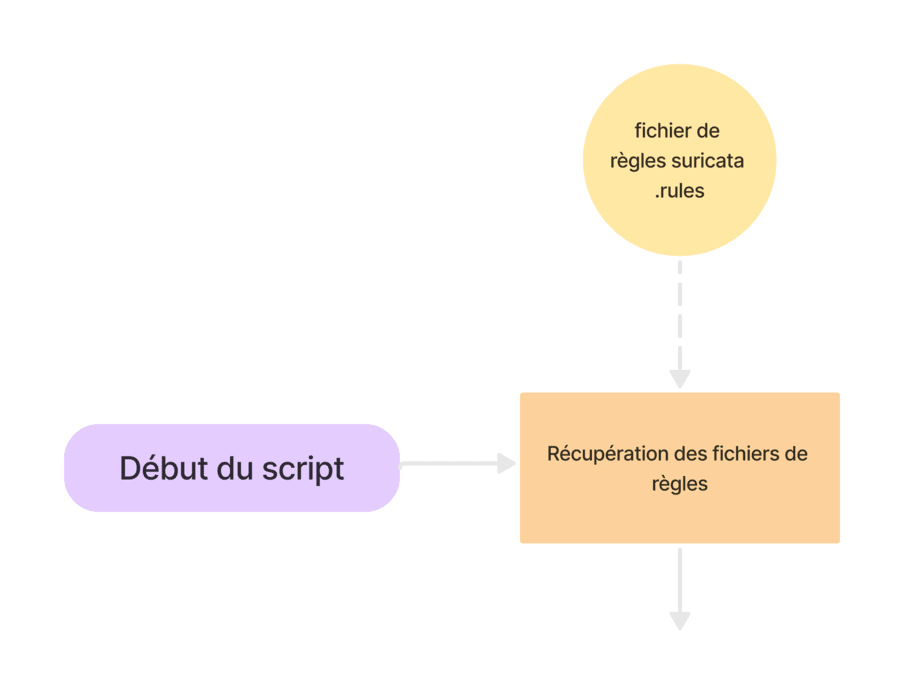
\includegraphics[width=0.7\textwidth]{assets/diagrameFlux3-1.png}
    \caption[Diagramme de flux de la section responsable de la récupération des règles]{Diagramme de flux de la section responsable de la récupération des règles}\label{fig:diagrameFlux3-1}
\end{figure}

\vspace{1em}

Le script a été conçu pour récupérer en entrée un dossier positionné à la racine du programme avec les fichiers de règles qui seront lus par le programme.\\

\begin{figure}[h]%
    \center%
\begin{lstlisting}[language=Python]
# Parcours chaque fichier dans le repertoire fourni
for filepath in os.listdir("rules"):
    suricata_alerts = extract_suricata_alerts(filepath)
\end{lstlisting}
    {\small
    \textit{Traite chaque fichier de règles individuellement depuis le dossier "rules"}
    }
    \caption[Récupération des règles]{Récupération des règles}
\end{figure}

Chaque fichier présent dans le dossier va être testé puis ensuite les règles seront récupérées et rassemblées.

\newpage

\subsection{Contrôle des règles en entrée}

\vspace{1em}

Avant la récupération des règles, le programme doit être capable de tester les règles récupérées car selon les retours des membres du CERT-MC, il arrivait que des erreurs (faute de frappe, mauvaise valeur inscrite...) soient contenues dans les règles de détection des fichiers récupérés ou que lesdites règles soient destinées à une version de Suricata qui n'est pas compatible avec celles des sondes. Ce qui pouvait provoquer le blocage d'une sonde si les règles en question arrivaient en bout de chaîne.\\

\vspace{0.5em}

Pour cette raison il était attendu de mon programme qu'il soit capable de contrôler la validité des règles avec les sondes pour prévenir, en cas de panne, le risque de perte en capacité de détection.\\

\begin{figure}[h]%
    \center%
    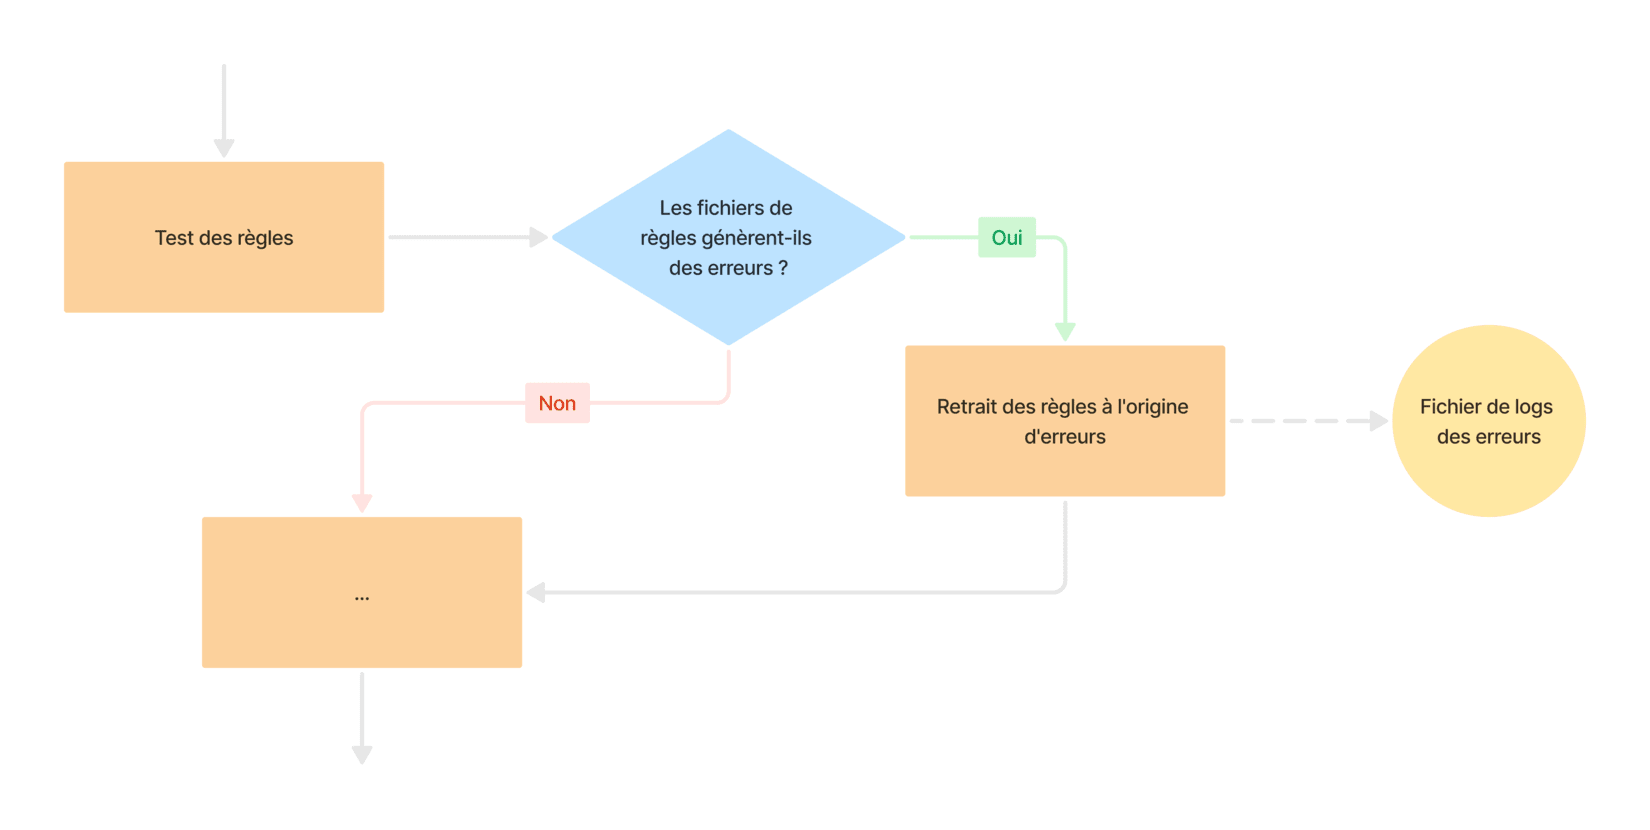
\includegraphics[width=1\textwidth]{assets/diagrameFlux3-2.png}
    \caption[Diagramme de flux de la section responsable du contrôle des règles]{Diagramme de flux de la section responsable du contrôle des règles}\label{fig:diagrameFlux3-2}
\end{figure}

\vspace{1em}

Le programme va ainsi tester individuellement chaque fichier récupéré. Pour cela Suricata dispose d'un mode test qui permet de compiler un fichier de règles. A cette fin, une version de Suricata comparable à celle présentée sur les sondes a été installée localement sur mon poste de travail. 

\newpage

\begin{figure}[h]%
    \center%
\begin{lstlisting}[language=Python]
testresult = subprocess.run(['suricata', '-T', '-c', 'configTestSuricata.yaml','-l', '/tmp/', '-S', filepath], capture_output=True, text=True)
\end{lstlisting}
    {\small
    \textit{Teste le fichier présent dans la variable "filepath" en utilisant la version locale de Suricata et le fichier de configuration 'configTestSuricata.yaml’ \hyperref[chap:annexe1]{[A.1]}}
    }
    \caption[Test des fichiers de règles]{Test des fichiers de règles}\label{fig:TestFileRule}
\end{figure}

\vspace{1em}

Pour chaque fichier testé, la version locale de Suricata génère des journaux d'erreurs qui désignent chaque règle ayant provoqué des erreurs avec une description de celle-ci \hyperref[chap:annexe2]{[A.2]}. A partir de ces journaux des résultats des tests, j'identifie les potentielles règles défectueuses.\\

\begin{figure}[h]%
    \center%
    \begin{lstlisting}[language=Python]
# Si le fichier produit une erreur
if (testresult.returncode == 1):
    # 'stderr' = toute les erreurs qui ont encourue
    for line in testresult.stderr.split('\n'):
        if line.startswith('E: detect: error parsing signature'):
            # Extraction de la ligne des messages d'erreur
            linenumber = line.split(' ')[-1]
            line_to_remove.append(int(linenumber))
            # Recuperation des erreurs pour creation csv
            csvError["collumnRules"].append(line)
        else:
            csvError["collumnError"].append(line)
\end{lstlisting}
    {\small
    \textit{Parcours de chaque ligne des journaux d'erreurs pour dénombrer les lignes non fonctionnelles. "Linenumber" est la variable qui stocke les numéros des lignes des règles qui provoquent des erreurs.}
    }
    \caption[Identification des règles ayant provoqué des erreurs]{Identification des règles ayant provoqué des erreurs}\label{fig:IdentRulesError}
\end{figure}

\vspace{1em}

Celles-ci seront mises de côté pour la prochaine mise à jour des sondes pour n'utiliser que les valides pour le reste du programme.\\

\begin{figure}[h]%
    \center%
    \begin{lstlisting}[language=Python]
# Boucle dans les fichiers de regles
with open(filepath, 'r') as file:
    for i, line in enumerate(file, start=1):
        # On ne garde que les lignes qui ne font pas partie des erreurs
        if i not in line_to_remove and line.startswith("alert "):
            suricata_alerts.append({'rules': line, 'source': sourceName})

return suricata_alerts
\end{lstlisting}
    {\small
    \textit{Parcours à nouveau du fichier de règles testé, en supprimant toutes les lignes qui ont été détectées comme étant à l'origine d'erreurs. "suricata\_alerts", les règles finales récupérées.}
    }
    \caption[Récupération des règles en excluant les erreurs]{Récupération des règles en excluant les erreurs}\label{fig:GetRules}
\end{figure}

\newpage

Afin de pouvoir tenir compte des règles qui commettent des erreurs au fil du temps, celles-ci sont stockées dans des fichiers CSV (Figure 3.12) avec leur code d'erreur. Cela permet d'établir des statistiques sur le taux de règles valides envoyées par les partenaires de renseignement sur la menace.\\

\subsubsection{\textit{Note}}
Le format CSV a été choisi pour stocker les informations relatives aux fichiers de configuration et aux résultats du programme. Ce format est utilisé parce qu'il est compatible avec Excel et Splunk, deux logiciels largement utilisés au sein de l'Agence.

\newpage

\subsection{Filtrage des règles}

\vspace{1em}

Une fois que les règles non valides ont été supprimées de l'ensemble traité, un autre problème se pose. Par la multitude de fournisseurs de règles, il existe le risque que la même règle (ayant probablement été établie à partir du même IOC) soit partagée par plusieurs partenaires différents. C'est pourquoi, pour éviter la surcharge inutile des sondes, il m'a été demandé de permettre à l'outil développé de filtrer les règles dupliquées.\\

\begin{figure}[h]%
    \center%
    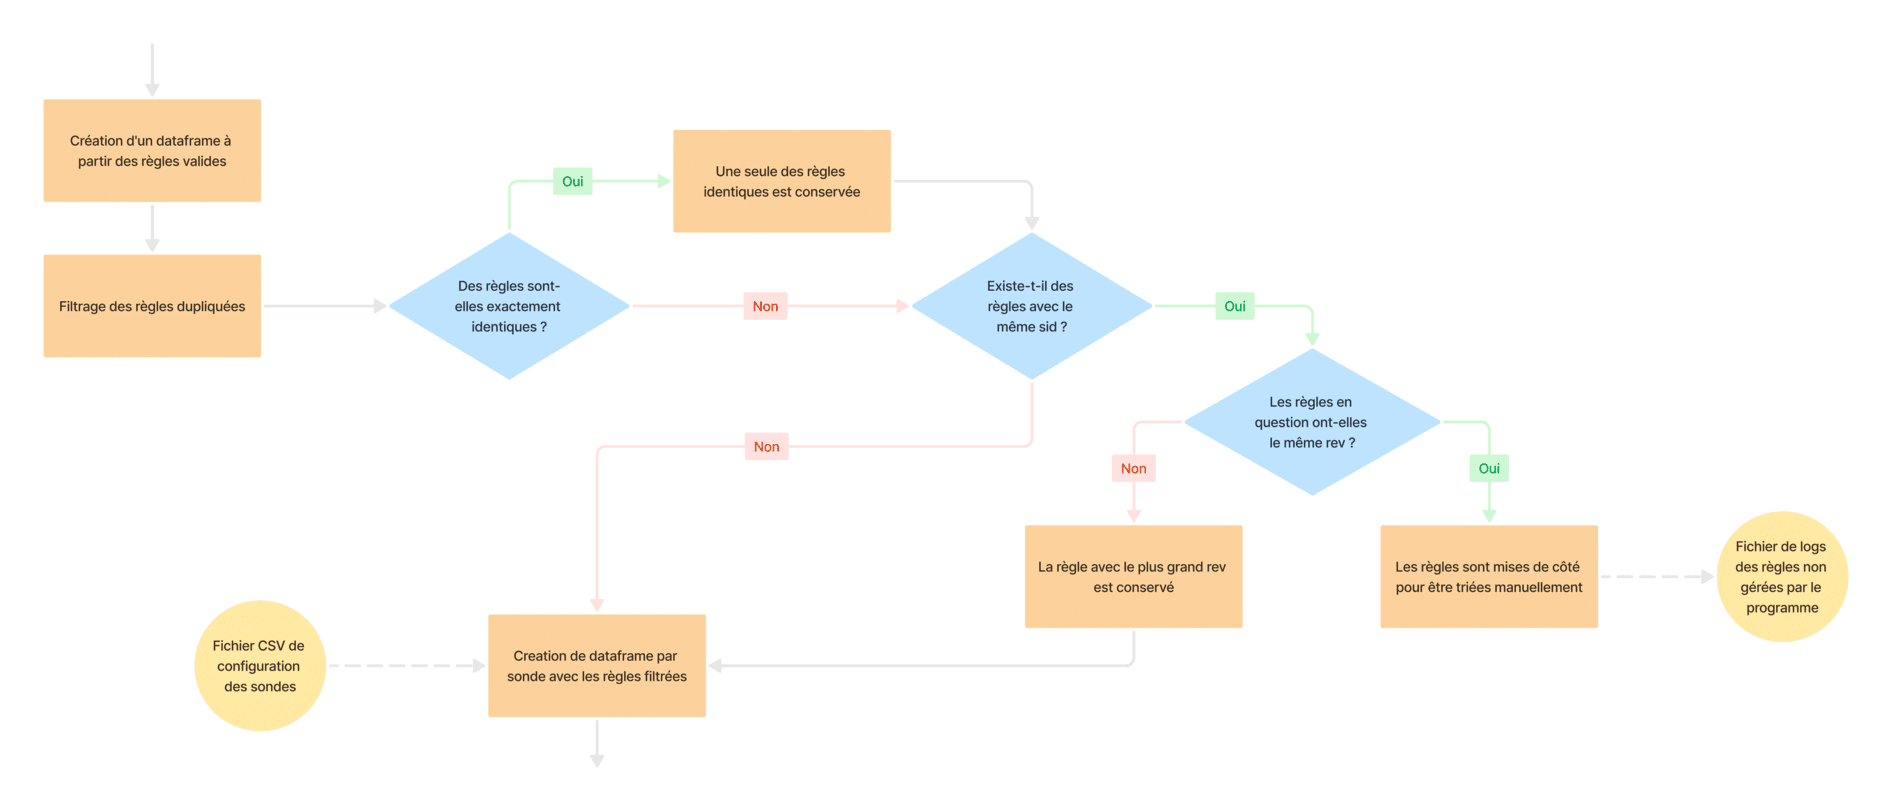
\includegraphics[width=1\textwidth]{assets/diagrameFlux3-3.png}
    \caption[Diagramme de flux de la section responsable du filtrage des règles]{Diagramme de flux de la section responsable du filtrage des règles}\label{fig:diagrameFlux3-3}
\end{figure}

\vspace{1em}

Pour mener à bien cette tâche (ainsi que d'autres manipulations que le programme devra appliquer à ces données par la suite), j'ai eu besoin d'utiliser une bibliothèque logicielle de data-science : \textit{pandas}\footnote{Pandas est une bibliothèque open-source flexible d'analyse et de manipulation de données pour Python : \url{https://pandas.pydata.org/}}. Elle permet de créer des ensembles de structures de données bidimensionnelles, \textit{dataframes}, qui permettent au programme de rassembler toutes les règles dans une seule variable et d'appliquer des modifications à l'ensemble en quelques lignes de code seulement.\\

\newpage

\begin{figure}[h]%
    \center%
\begin{lstlisting}[language=Python]
#Import de la librairie
import pandas as pd

Dataframe_alerts = pd.DataFrame(suricata_alerts)
\end{lstlisting}
    {\small
    \textit{Importation de la bibliothèque Pandas et création d'un \textit{dataframe} à partir de "suricata\_alerts", une liste composée de toutes les règles récupérées jusqu'à présent.}
    }
    \caption[Création de dataframe \textit{pandas}]{Création de dataframe \textit{pandas}}\label{fig:CreateDataf}
\end{figure}

\subsubsection{\textit{Note}}
J'avais initialement essayé de réaliser ce programme en utilisant uniquement les outils fournis par défaut par Python, mais la taille colossale des données à traiter (plusieurs dizaines de milliers de règles) a rendu cette option inefficace et a provoqué un ralentissement excessif de l'exécution du programme. Cela m'a contraint à recourir à des outils de traitement de données. Le choix s'est porté sur Pandas car il s'agit d'une bibliothèque reconnue pour sa performance et qui est régulièrement maintenue.\\

\vspace{0.5em}

Grâce à cette bibliothèque, le processus de filtrage s'est déroulé en deux étapes. Tout d'abord, les règles qui sont strictement identiques à d'autres sont supprimées.\\

\begin{figure}[h]%
    \center%
\begin{lstlisting}[language=Python]
# Trouve toutes les regles strictement en double pour n'en garder qu'une
duplicates = allrules[allrules.duplicated('rules', keep=False)]
if duplicates.empty == False:
    grouped = duplicates.groupby('rules')['source'].agg(', '.join).reset_index()
    allrules = pd.concat([allrules[~allrules['rules'].isin(duplicates['rules'])], grouped], ignore_index=True)
\end{lstlisting}
    \caption[Suppression des règles dupliquées]{Suppression des règles dupliquées}\label{fig:DeleteRules}
\end{figure}

\vspace{1em}

Puis elles sont triées en fonction du \textit{sid} et de la \textit{rev} des règles.
Cette seconde étape est due au fonctionnement de Suricata qui exige que la section \textit{options} des règles comporte une variable \textit{sid} (pour signature ID) unique à chaque règle, qui est utilisée pour les identifier. Comme les partenaires de l'Agence respectent les conventions d'écriture des règles et en particulier les plages d'allocation de \textit{sid}\footnote{\url{https://sidallocation.org/}}, différentes règles ayant le même \textit{sid} sont nécessairement basées sur le même IOC et le programme n'a plus qu'à décider lequel conserver.\\

\newpage

Pour départager deux règles ayant le même \textit{sid}, j'utilise une autre variable présente dans les options des règles Suricata \textit{rev} (pour revision) qui sert à spécifier un numéro de version d'une règle. La règle ayant la valeur numérique de sa variable \textit{rev} la plus élevée est la règle qui à été mise à jour en dernier et sera donc privilégiée.\\

\vspace{0.5em}

\begin{figure}[h]%
    \center%
\begin{lstlisting}[language=Python]
# On ceer une collone sid dans le dataframe a partir des sid des regles
allrules['sid'] = allrules['rules'].str.extract(r'sid:(.*?);')

# On trouve toutes les sid n'etant pas unique dans le dataframe
conflictedrules = allrules[allrules.duplicated('sid', keep=False)]

# Creation d'une nouvelle collone rev pour priorisation par rev
conflictedrules['rev'] = conflictedrules['rules'].str.extract(r'rev:(.*?);').astype(int)
# Groupe par 'sid'
grouped = conflictedrules.groupby('sid')
# Groupe par 'rev'
max_rev_per_group = grouped['rev'].max()

# Garde pour chaque sid la regle ayant la plus haute rev. si des regle on la meme sid et rev elles seront non resolu
conflictedrules = conflictedrules[conflictedrules.apply(lambda x: x['rev'] == max_rev_per_group[x['sid']], axis=1)]
\end{lstlisting}
    \caption[Gestions des règles en collision de sid]{Gestions des règles en collisions de sid}\label{fig:HandlingCollisions}
\end{figure}

\vspace{0.5em}

Une fois le tri terminé, de nouveaux \textit{dataframmes} sont créés pour correspondre au nombre de sondes qui recevront des fichiers de règles en sortie du programme. Ces différents \textit{dataframmes} sont utilisés pour appliquer des modifications aux règles en fonction des sondes cibles.

\vspace{1em}

\begin{figure}[h]%
    \center%
\begin{lstlisting}[language=Python]
# creer un dataframes de regles pour chaque sonde
rulesByProbes = {}
for name in SondesNames:
   rulesByProbes[name[0]] = cleanedrules[:]
\end{lstlisting}
{\small
    \textit{Crée un dictionnaire d'images de données pour chaque sonde finale.}
    }
    \caption[Création de dataframe pour chaque sonde]{Création de dataframe pour chaque sonde}\label{fig:CreateDatafBySonde}
\end{figure}

\newpage

\subsection{Modification des règles}
\label{chap3:section1rulesmodif}

\vspace{1em}

Les membres du SOC-MC m'avaient fait part de leur besoin d'acquérir la capacité de modifier facilement les ensembles de règles. Les analystes du SOC-MC observent lors de leur travail quotidien l'efficacité des règles mises en place sur les sondes. Leurs observations et enquêtes ont mis en évidence des règles inutiles ou trop "bruyantes" que mon programme devait être capable de modifier.

\begin{figure}[h]%
    \center%
    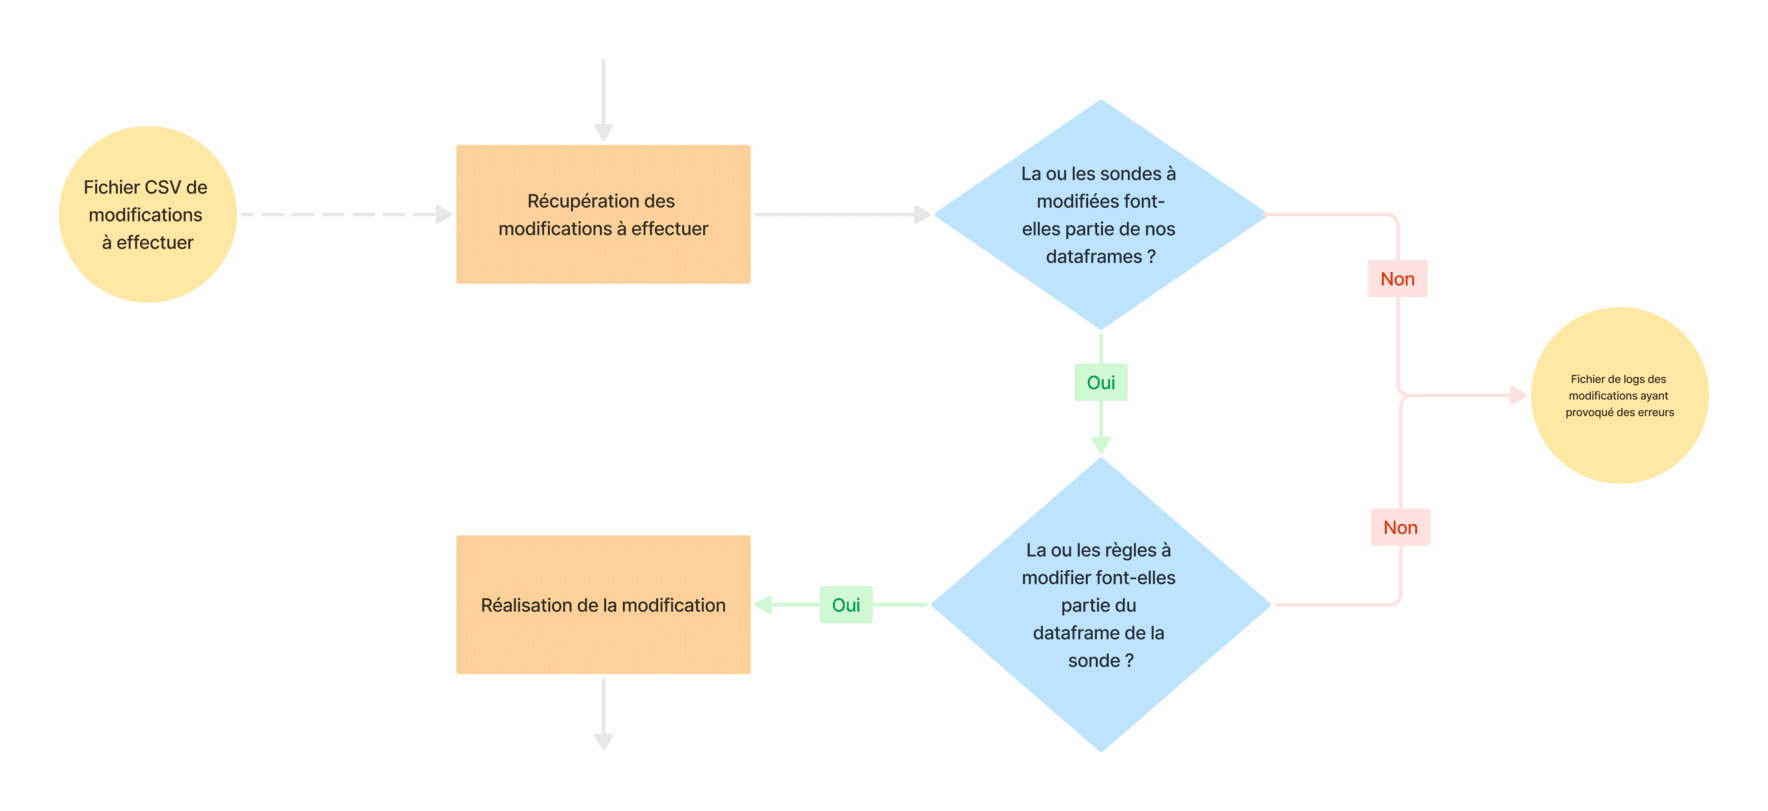
\includegraphics[width=1\textwidth]{assets/diagrameFlux3-4.png}
    \caption[Diagramme de flux de la section responsable de l'application des modifications]{Diagramme de flux de la section responsable de l'application des modifications}\label{fig:diagrameFlux3-4}
\end{figure}

\vspace{1em}

Les modifications à effectuer sont fournies au programme sous la forme d'un fichier CSV stipulant les règles à rectifier en fonction de leur \textit{sid} ainsi que l'amendement à apporter et pour quelle sonde l'appliquer. Ce fichier est complété soit par les analystes SOC, soit par d'autres membres du CERT-MC sur la base de leurs constatations quant à l'efficacité des règles sur les sondes.\\

\vspace{1em}

\begin{figure}[h]%
    \center%
    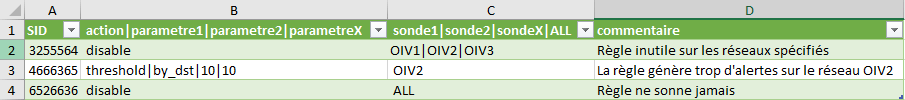
\includegraphics[width=1\textwidth]{assets/CaptureCSV.png}
    \caption[Exemple de fichier CSV de configuration des règles à modifier]{Exemple de fichier CSV de configuration des règles à modifier}\label{fig:CaptureCSV}
\end{figure}

\newpage

Le programme récupère le contenu du fichier et désactive les règles ou applique des seuils pour réduire le nombre d'alertes qu'elles génèrent (des "threshold" dans la terminologie de Suricata).\\

\begin{figure}[h]%
    \center%
\begin{lstlisting}[language=Python]
# On applique la modification
if (changeToApply == "disable"):
    # Pour 'disable' on enleve la regle de la liste
    rulesByProbes[sonde[0]] = rulesByProbes[sonde[0]][rulesByProbes[sonde[0]]["sid"] != targetSid]
elif len(changeToApply) > 3:
    # Hors 'disable' il s'agit d'un changement de threshold
    # On cree la nouvelle option
    changeToApply = "threshold: type " + changeToApply[0] + ", track " + changeToApply[1] + ", seconds " + changeToApply[3] + ", count " + changeToApply[2] + ";"
    # rulesToChange = la regle qui va etre modifiee
    rulesToChange = rulesByProbes[sonde[0]].loc[rulesByProbes[sonde[0]]["sid"] == targetSid, 'rules']
    # On modifie la section msg de la regle pour notifier qu'elle a ete modifiee
    rulesToChange = rulesToChange.str.replace('msg:"', 'msg:"AMSN_RULE ')
    # Si l'option threshold existe deja dans rulesToChange on la remplace par la nouvelle
    if (re.search('threshold:', rulesToChange.tolist()[0])):
        rulesToChange = rulesToChange.str.replace(r'threshold:(.*?);', changeToApply, regex=True)
    # S'il n'y a pas d'option threshold dans la regle modifiee on place la nouvelle option a la fin 
    else:
        rulesToChange = rulesToChange.values[0].rsplit(')', 1)[0] + changeToApply + ')\n'
    # on reincopore la regle modifiee dans le dataframe de la sonde selectionnee
    rulesByProbes[sonde[0]].loc[rulesByProbes[sonde[0]]["sid"] == targetSid, 'rules'] = rulesToChange
\end{lstlisting}
{\small
    \textit{Modifie les règles en écrivant à l'intérieur les nouvelles valeurs dans le cas de changement de 'threshold' et retire la règle du dataframe dans le cas d'un changement 'disable'.}
    }
\caption[Modifications des règles]{Modifications des règles}\label{fig:ModifRules}
\end{figure}

\vspace{1em}

Ces seuils sont une option activée par Suricata, permettant de limiter le nombre d'alertes par minute générées par une règle. Les modifications ne sont apportées qu'aux \textit{dataframes} destinés aux sondes spécifiées dans le fichier CSV, permettant une différenciation par OIV.

\newpage

\subsection{Traitement des résultats}

\vspace{1em}

Afin de répondre aux exigences de l'Agence, le programme doit utiliser les opérations précédentes pour générer un fichier de règles, pour chaque sonde destinataire, qui puisse être exporté facilement. En outre, pour permettre à l'Agence de suivre les résultats du programme dans le temps, j'ai dû mettre en place un système de journalisation dans le code.

\begin{figure}[h]%
    \center%
    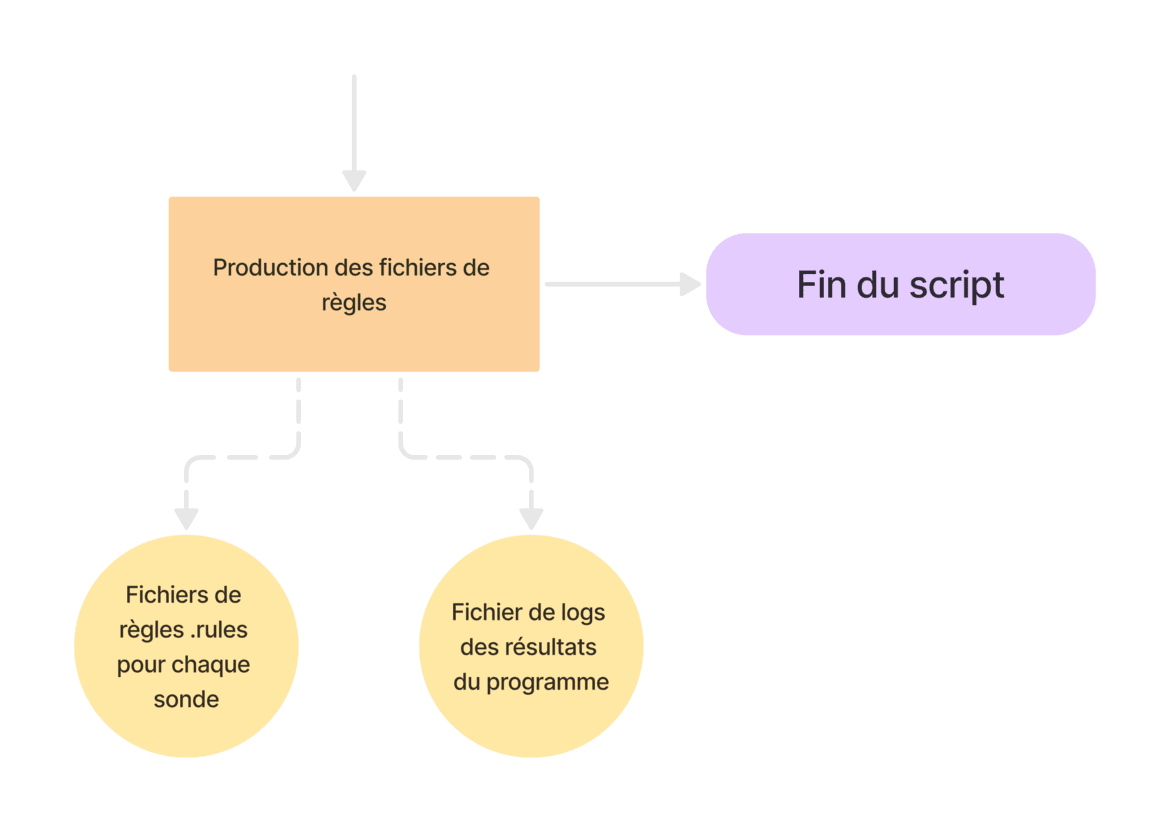
\includegraphics[width=0.8\textwidth]{assets/diagrameFlux3-5.png}
    \caption[Diagramme de flux de la fin du programme]{Diagramme de flux de la fin du programme}\label{fig:diagrameFlux3-5}
\end{figure}

\vspace{1em}

À partir des \textit{dataframes} mentionnés précédemment, un fichier de règles a été généré pour chaque sonde et est stocké dans un dossier distinct afin de pouvoir être exporté vers le système de gestion des sondes.\\

\newpage

\begin{figure}[h]%
    \center%
\begin{lstlisting}[language=Python]
### AMSN generated rules files ###

alert udp any any -> $HOME_NET 139 (msg:"ET NETBIOS Microsoft Windows NETAPI Stack Overflow Inbound - MS08-067 (1)"; content:"|0B|"; offset:2; depth:1; content:"|C8 4F 32 4B 70 16 D3 01 12 78 5A 47 BF 6E E1 88|"; reference:url,www.microsoft.com/technet/security/Bulletin/MS08-067.mspx; reference:cve,2008-4250; reference:url,www.kb.cert.org/vuls/id/827267; classtype:attempted-admin; sid:2008690; rev:5;  metadata: amsn_source gcenter_netbios, created_at 2010_07_30, cve CVE_2008_4250, updated_at 2017_11_22;)

alert tcp $EXTERNAL_NET any -> $HOME_NET 139 (msg:"ET NETBIOS Microsoft SMB NetLogon UUID detected Big Endian SET"; flow:to_server,established; content:"|ff|SMB"; content:"|05 00 0b|"; distance:0; byte_test:1,!&,0x10,1,relative; content:"|12345678 1234 abcd ef00 01234567cffb|"; distance:29; flowbits:set,smb.netlogon.uuid.detected; flowbits:noalert; reference:cve,2010-2742; reference:url,www.microsoft.com/technet/security/bulletin/MS10-101.mspx; classtype:attempted-user; sid:2800985; rev:2;  metadata: amsn_source gcenter_netbios, created_at 2010_12_15, cve CVE_2010_2742, updated_at 2017_11_22;)

...
\end{lstlisting}
    \caption[Exemple de fichier de règles généré]{Exemple de fichier de règles généré}\label{fig:captureOIVrules}
\end{figure}

\vspace{1em}

Pour pouvoir répondre au besoin d'information sur les résultats du programme, j'ai mis en place une journalisation via la génération de CSV tout au long de l'exécution du programme :\\

\vspace{1em}

\begin{itemize}[itemsep=2em]
    \item[•] Lorsque les règles récupérées sont testées, un fichier CSV est créé pour enregistrer les règles qui ont été détectées comme étant à l'origine d'erreurs et leurs sources.

\vspace{1em}

    \begin{figure}[h]%
        \center%
        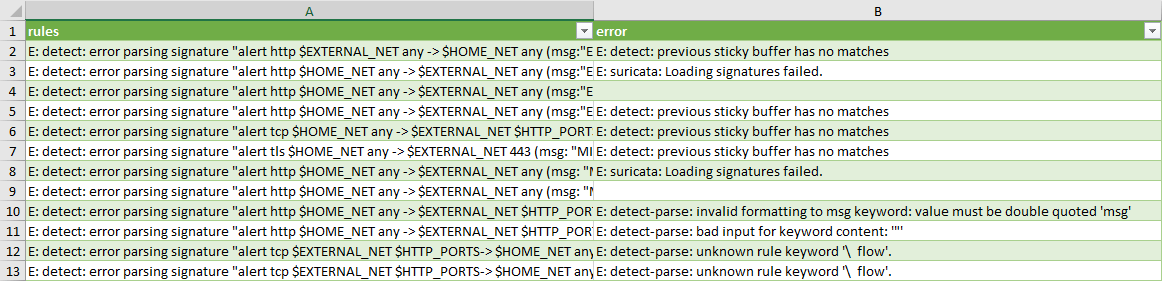
\includegraphics[width=0.9\textwidth]{assets/SuricataError.png}
        \caption[Exemple de fichier CSV d'erreurs dans les fichiers testés]{Exemple de fichier CSV d'erreurs dans les fichiers testés}\label{fig:SuricataError}
    \end{figure}

\newpage

    \item[•] Lorsque les règles en double sont filtrées, un fichier CSV est créé pour les règles potentielles qui ne peuvent pas être gérées automatiquement en vue d'un tri manuel.

\vspace{1em}

    \begin{figure}[h]%
        \center%
        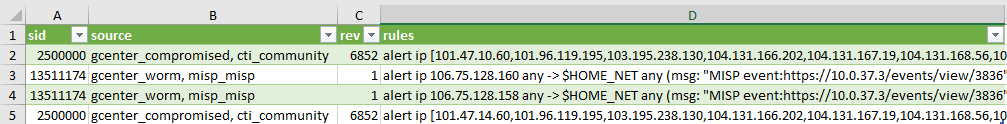
\includegraphics[width=1\textwidth]{assets/RuleColision.png}
        \caption[Exemple de fichier CSV de règles dupliquées non géré]{Exemple de fichier CSV de règles dupliquées non gérées}\label{fig:RuleColision}
    \end{figure}

    \item[•] Lorsque les modifications demandées par le personnel du CERT-MC sont appliquées, les modifications qui n'ont pas pu être effectuées (en raison d'une erreur dans les fichiers de configuration) sont sauvegardées dans un fichier CSV.\\

\vspace{1em}

    \begin{figure}[h]%
        \center%
        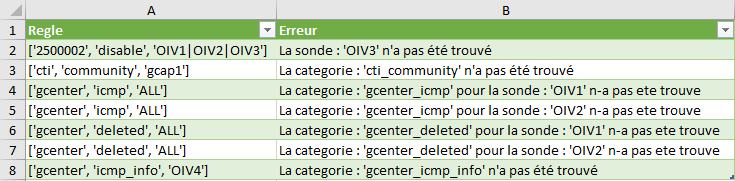
\includegraphics[width=0.8\textwidth]{assets/ErrorModif.png}
        \caption[Exemple de fichier CSV d'erreur de modification de règle]{Exemple de fichier CSV d'erreur de modification de règle}\label{fig:ErrorModif}
    \end{figure}

\vspace{1em}

    \item[•] Lorsque le programme est terminé, un fichier de statistiques générales est généré.\\

\newpage

    \begin{figure}[h]%
        \center%
        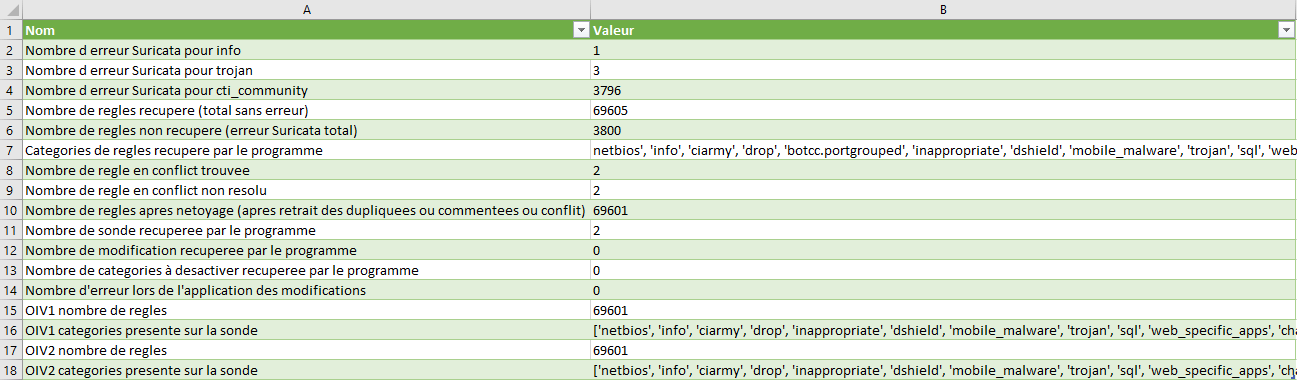
\includegraphics[width=1\textwidth]{assets/stat.png}
        \caption[Exemple de fichier CSV de statistiques du programme]{Exemple de fichier CSV de statistiques du programme}\label{fig:Stat}
    \end{figure}

\end{itemize}

\vspace{1em}

Ces fichiers sont générés à chaque mise à jour des sondes et sont stockés séparément par date. Les fichiers ainsi créés permettent de comparer les résultats des différentes mises à jour des sondes et de suivre dans le temps quelles règles étaient actives sur chaque sonde à un moment donné.\\

L'importance de développer cette capacité est de permettre au programme de répondre à certaines exigences du référentiel \textit{PDIS}\footnote{\textit{"Le prestataire doit élaborer et tenir à jour pour chaque commanditaire la liste de l’ensemble des règles de détection mises en œuvre ou ayant été mises en œuvre dans le cadre de la prestation."} \hyperref[biblio]{[9]}} de l'ANSSI auxquelles l'ancien processus d'alimentation des sondes ne pouvait répondre.\\

\vspace{1em}

\subsubsection{\textit{Note}}
Le développement de ce code a duré environ un mois et demi, comprenant la production de tests unitaires et de documentation, suivi d'une période de vérification du code par mon tuteur de stage et la planification de la mise en production du programme. Au moment de la publication de ce document, le programme est effectivement utilisé dans les processus courants de l'Agence.